% DDS  3 : COMMENCER à 169

\renewcommand{\repExo}{\repExos/C2_MettreEnOeuvreDemarche/C2_09_DeterminerLoiMouvement1D}
\setcounter{numexo}{168}
\renewcommand{\td}{61_Hemostase_02}
\graphicspath{{\repStyle/png/}{\repExo/\td/images/}}
\input{\repExo/\td/\td.tex}

\renewcommand{\repExo}{\repExos/C2_MettreEnOeuvreDemarche/C2_06_DeterminerLoisES}
\setcounter{numexo}{167}
\renewcommand{\td}{17_4Barres}
\graphicspath{{\repStyle/png/}{\repExo/\td/images/}}
\input{\repExo/\td/\td.tex}

\renewcommand{\repExo}{\repExos/C2_MettreEnOeuvreDemarche/C2_06_Transmetteurs}
\setcounter{numexo}{166}
\renewcommand{\td}{27_TrainEpi}
\graphicspath{{\repStyle/png/}{\repExo/\td/images/}}
\input{\repExo/\td/\td.tex}

\renewcommand{\repExo}{\repExos/C2_MettreEnOeuvreDemarche/C2_06_Transmetteurs}
\setcounter{numexo}{165}
\renewcommand{\td}{28_TrainEpi}
\graphicspath{{\repStyle/png/}{\repExo/\td/images/}}
\input{\repExo/\td/\td.tex}

\renewcommand{\repExo}{\repExos/C2_MettreEnOeuvreDemarche/C2_06_Transmetteurs}
\setcounter{numexo}{164}
\renewcommand{\td}{31_Redex}
\graphicspath{{\repStyle/png/}{\repExo/\td/images/}}
\input{\repExo/\td/\td.tex}

\renewcommand{\repExo}{\repExos/C2_MettreEnOeuvreDemarche/C2_06_Transmetteurs}
\setcounter{numexo}{163}
\renewcommand{\td}{36_VisEcrou}
\graphicspath{{\repStyle/png/}{\repExo/\td/images/}}
\input{\repExo/\td/\td.tex}

\renewcommand{\repExo}{\repExos/C2_MettreEnOeuvreDemarche/C2_06_DeterminerLoisES}
\setcounter{numexo}{162}
\renewcommand{\td}{18_Maxpid}
\graphicspath{{\repStyle/png/}{\repExo/\td/images/}}
\input{\repExo/\td/\td.tex}

\renewcommand{\repExo}{\repExos/B2_ProposerModele/B2_13_ModeliserCinematique}
\setcounter{numexo}{161}
\renewcommand{\td}{06_TR_02}
\graphicspath{{\repStyle/png/}{\repExo/\td/images/}}
\input{\repExo/\td/\td.tex}

\renewcommand{\repExo}{\repExos/B2_ProposerModele/B2_13_ModeliserCinematique}
\setcounter{numexo}{160}
\renewcommand{\td}{07_RR3D_02}
\graphicspath{{\repStyle/png/}{\repExo/\td/images/}}
\input{\repExo/\td/\td.tex}

\renewcommand{\repExo}{\repExos/B2_ProposerModele/B2_13_ModeliserCinematique}
\setcounter{numexo}{159}
\renewcommand{\td}{09_RT_RSG}
\graphicspath{{\repStyle/png/}{\repExo/\td/images/}}
\input{\repExo/\td/\td.tex}

\renewcommand{\repExo}{\repExos/B2_ProposerModele/B2_13_ModeliserCinematique}
\setcounter{numexo}{158}
\renewcommand{\td}{12_BielleManivelle}
\graphicspath{{\repStyle/png/}{\repExo/\td/images/}}
\input{\repExo/\td/\td.tex}

\renewcommand{\repExo}{\repExos/C2_MettreEnOeuvreDemarche/C2_03_PerformancesSLCI_Precision}
\setcounter{numexo}{157}
\renewcommand{\td}{64_EPAS}
\graphicspath{{\repStyle/png/}{\repExo/\td/images/}}
\input{\repExo/\td/\td.tex}

\begin{center}
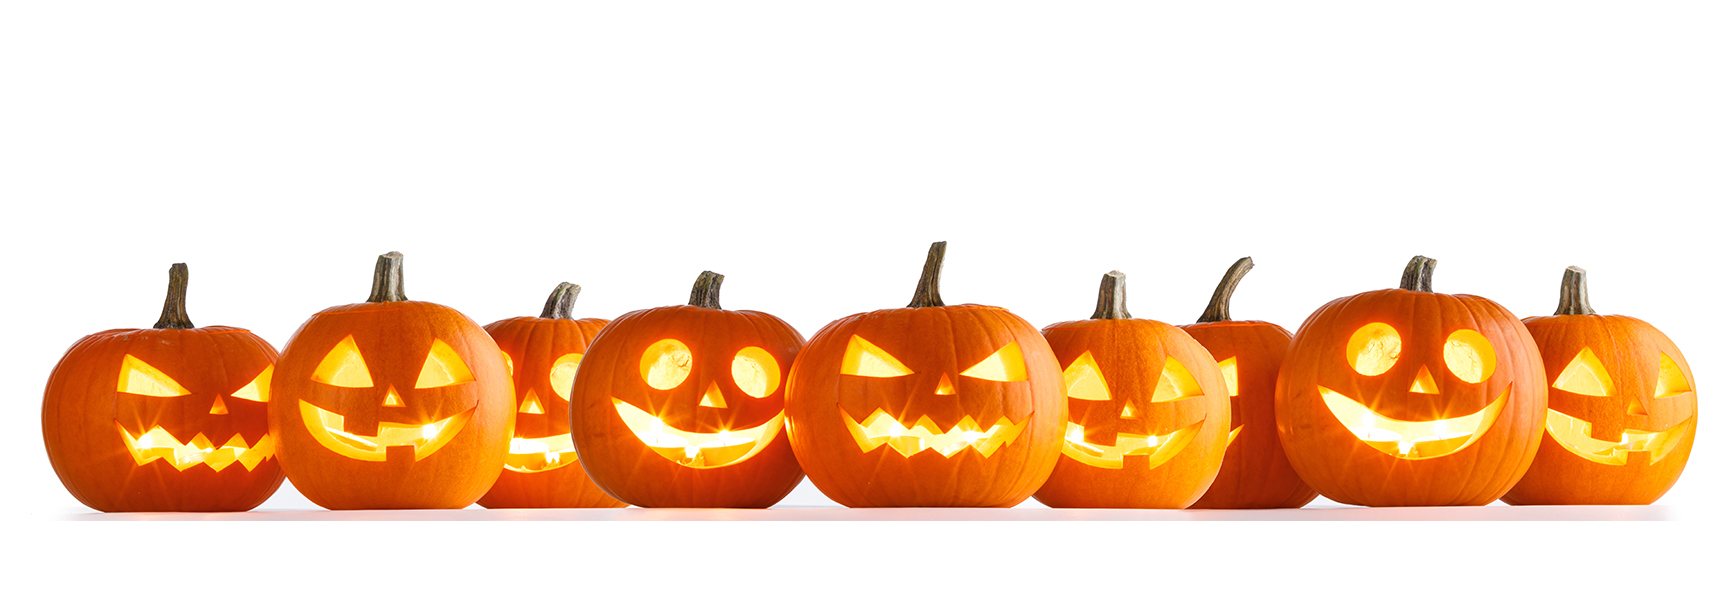
\includegraphics[width=\linewidth]{citrouilles}
\end{center}

\renewcommand{\repExo}{\repExos/C2_MettreEnOeuvreDemarche/C2_03_PerformancesSLCI_Stabilite}
\setcounter{numexo}{156}
\renewcommand{\td}{64_EPAS}
\graphicspath{{\repStyle/png/}{\repExo/\td/images/}}
\input{\repExo/\td/\td.tex}

\renewcommand{\repExo}{\repExos/C2_MettreEnOeuvreDemarche/C2_06_DeterminerLoisES}
\setcounter{numexo}{155}
\renewcommand{\td}{64_EPAS}
\graphicspath{{\repStyle/png/}{\repExo/\td/images/}}
\input{\repExo/\td/\td.tex}

\renewcommand{\repExo}{\repExos/C2_MettreEnOeuvreDemarche/C2_07_PFS}
\setcounter{numexo}{154}
\renewcommand{\td}{64_EPAS}
\graphicspath{{\repStyle/png/}{\repExo/\td/images/}}
\input{\repExo/\td/\td.tex}

\renewcommand{\repExo}{\repExos/C2_MettreEnOeuvreDemarche/C2_03_PerformancesSLCI_Stabilite}
\setcounter{numexo}{153}
\renewcommand{\td}{61_Hemostase}
\graphicspath{{\repStyle/png/}{\repExo/\td/images/}}
\input{\repExo/\td/\td.tex}

\renewcommand{\repExo}{\repExos/C2_MettreEnOeuvreDemarche/C2_09_DeterminerLoiMouvement1D}
\setcounter{numexo}{152}
\renewcommand{\td}{61_Hemostase}
\graphicspath{{\repStyle/png/}{\repExo/\td/images/}}
\input{\repExo/\td/\td.tex}